\chapter{Project Presentation} \label{lab:project-presentation}


\section{Proposed Framework} \label{lab:ch4-proposed-framework}

The goal of this Masters' thesis is to provide a generic framework for a TOTP application on a USB stick, as well as an implementation for it.
In this section, we will focus on the framework, i.e., the ideas and principles, rather than the technology used.
The presented framework could work on other devices as well, it is a generic flow of actions meant to be abstract.
At the same time, the framework's main goal is security, so it has to take into account all kinds of attacks and countermeasures for them.
With all that in mind, the framework focuses on minimizing the possibility of exploits, errors, deadlocks.

Simply put, a TOTP application generates TOTP codes (numbers) based on TOTP secrets (Base32 codes).
The application which requires TOTP (example: Gmail, Facebook, etc.) displays a QR code or an equivalent secret.
The user scans the QR code or introduces the secret manually into the TOTP application, which usually runs on a personal mobile device.
From that point on, the TOTP application stores that secret in a way or other, and keeps generating TOTP codes.

The framework aims to replace the mobile device with a USB stick.
This goal shall be achieved by fulfilling the following requirements:
\begin{enumerate}
    \item
        \b{Generate TOTP codes}.
        This is the main functional requirement of the framework.
        TOTP code generation is a standard algorithm and requires only the current time and the TOTP secret.
    \item
        \b{Store the secrets safely}.
        TOTP secrets are sensitive information.
        They shall be stored in a way which is secure and resistant to possible cyber-attacks.
    \item
        \b{Keep the 2FA aspect}:
        The framework treats the device on which the app runs as the possession factor of Two-Factor Authentication.
        Breaking this aspect would make the framework useless.
\end{enumerate}

Figure \ref{fig:flows} shows the two main flows of the proposed architecture.
It proposes the combination of three secrets: a password for encrypting the USB stick (\b{disk encryption password}), a password for unlocking the application and encrypting the secrets (\b{user password}), and optionally a TPM-provided secret which is combined with the user password for extra security (\b{TPM secret}).
Each of these will be detailed in the following sections.  
The following sections will go in depth on each aspect.

\begin{figure}[htbp]
    \centering
    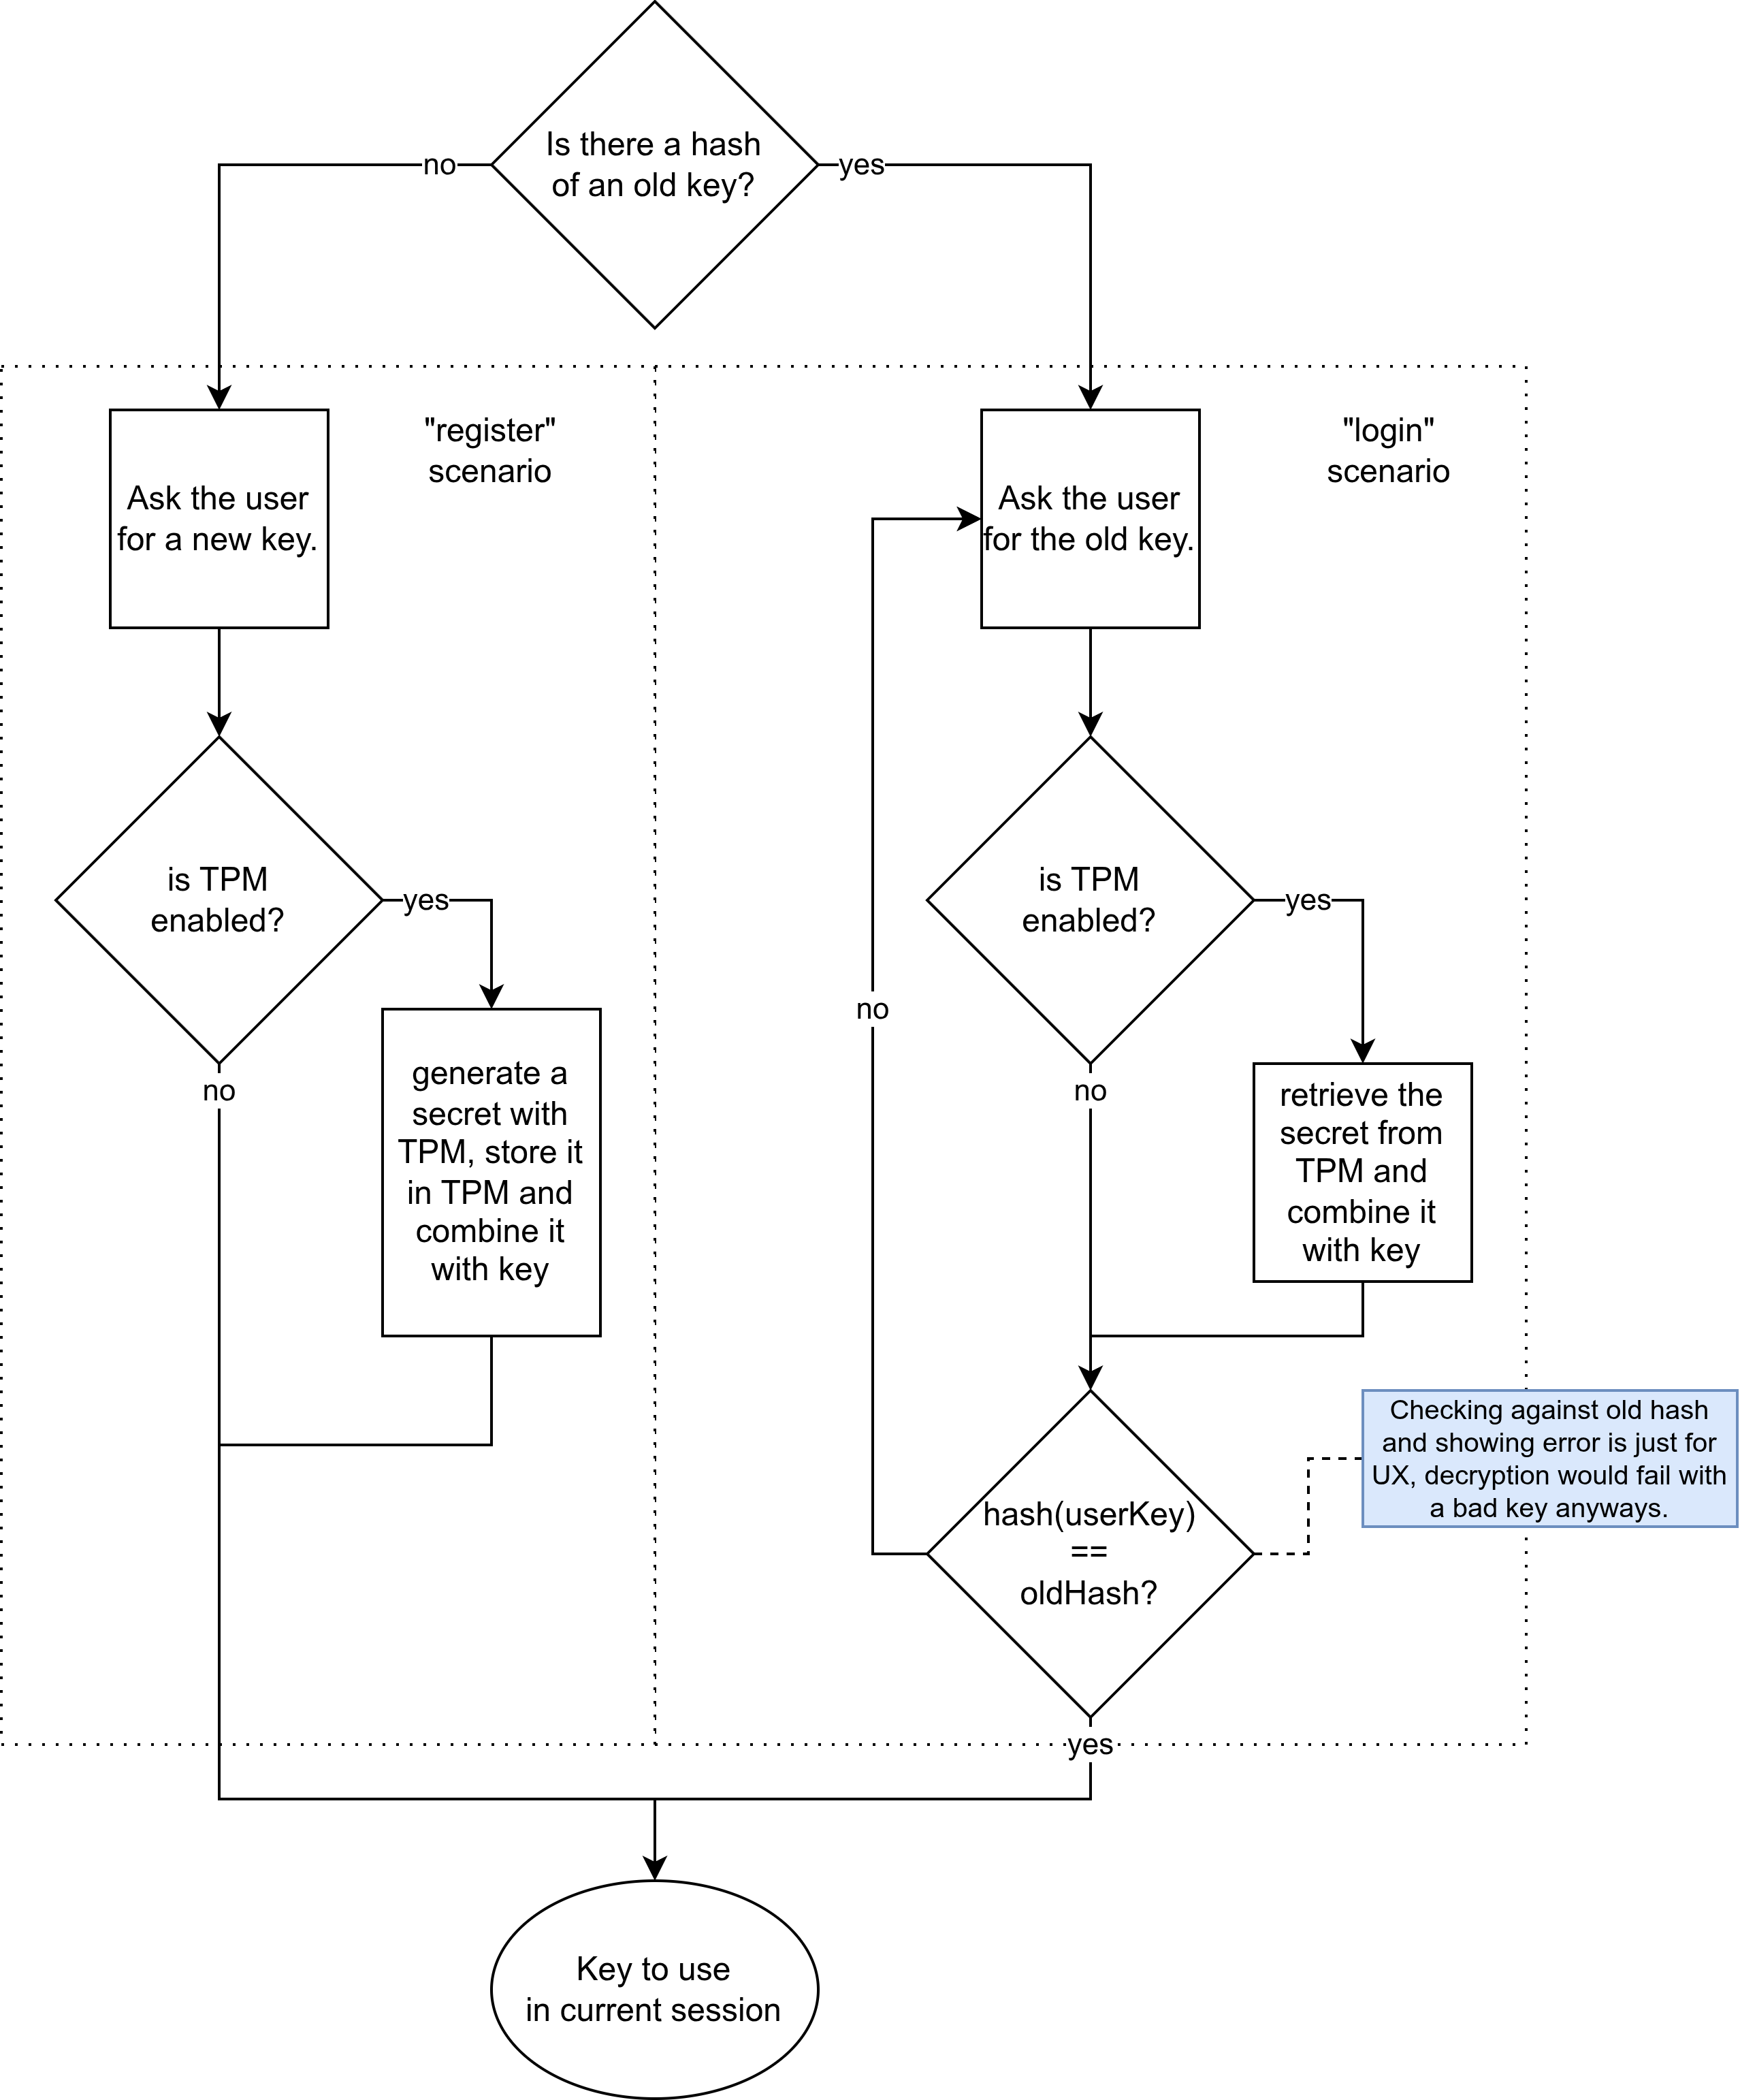
\includegraphics[width=\textwidth]{img/diagram-flows.png}
    \caption{The two main flows of the proposed framework.}
    \label{fig:flows}
\end{figure}

\subsection{Disk Encryption} \label{lab:ch4-disk-encryption}

The first line of defense is provided by the device on which the app resides: the USB itself shall be encrypted.
I will refer to the password used for the USB's encryption/ decryption as the \b{disk encryption password}.
Each operating system has specific USB formats and default disk encryption algorithms.
For Linux, Ext4 partition type encrypted with LUKS2 can be used (see: Section \ref{lab:ch3-luks}).
For Windows, W95 FAT32 partition type encrypted with BitLocker can be used.
The encryption of the device applies on its whole content.
This ensures that the stored secrets cannot be read without providing the disk encryption password.
Even if the running application saves passwords in plaintext, the USB encryption would encrypt it anyway.

The main issue of USB sticks (in our context) is that they are not read-only media.
Someone could steal the USB stick and copy its contents in less than a minute.
If the malicious actor puts the USB stick back to where he/she found it, the user would not even know.
The attacker could then brute-force breaking the USB without any time limitations.
Or even worse, if the attacker gets to know the disk encryption password, he/she can break in without having our media, using the copy.
Nevertheless, USB Encryption is a good first line of attack against not-so tech-savvy attackers.


\subsection{Storage Encryption} \label{lab:ch4-storage-encryption}

Aside of the password for the USB's encryption, the framework also requires a \b{user password}, for unlocking the application.
It is recommended for this password to be different from the password provided for the USB's encryption (see: Section \ref{lab:ch4-disk-encryption}), but a check for difference is out of scope.
So it is up to the user which user password it chooses, as long as it matches password complexity requirements.
The user password, aside of unlocking the application, is also used to encrypt the TOTP secrets the framework stores, in what we refer to as \b{storage}.

Of what use is another encryption on top of disk encryption?
You might ask, rightfully.
Well, disk encryption ensured data safety at rest, while the USB is locked, and storage encryption makes sure secrets are not stored in plaintext, even if the app is running and the USB is unlocked.
This protects against ``coffee-shop'' attacks: the user might leave their device unlocked and unsupervised.
In such cases, if the storage would be plaintext, an attacker could quickly read the secrets from their device.

Storage encryption is also a second layer of security on top of disk encryption.
While both could be brute-forced, if separate passwords are used for disk and storage encryption, the time required to do so increases.
While disk encryption algorithms might be more permissive regarding password complexity, and the framework has no control over it, the user password is required to be complex.
It is kind of a zero-trust scenario, where even if the user does not properly encrypt the disk it uses the framework on, the secrets are not leaked.

The user password is never stored.
Instead, the hash of the user password is stored inside a file, in what I refer to as the \b{hashed user password file}.
If the hashed user password file does not exist, the framework considers that no user password was provided beforehand.
The user is prompted to enter a new password.
This is the \b{register scenario}; although it is a one-user application, it is easier to refer to it with such standard naming.
If the hashed user password file exists at start, the framework considers that registering happened beforehand.
The user shall provide the old password, which is verified against the existing hash.
An incorrect password prevents the start of the flow, since the system has no knowledge about the password.
Without it, storage cannot be decrypted and secrets cannot be retrieved.


\subsection{Using TPM} \label{lab:ch4-using-tpm}

The read-write nature of a USB cannot be changed, and making a USB stick uncopiable is either impossible or out of scope.
The encryption with the help of the user password suffers the same vulnerability as the USB encryption, it is just another layer, but breakable in the same fashion.
Detecting if another TOTP Application is using the secret (for example, if the attacker stole the secret and introduced it into a TOTP application) is also out of scope.
However, the time required for brute-forcing can be made even bigger with the help of the Trusted Platform Module (TPM, see: Section \ref{lab:ch3-tpm}).

The framework proposes generating a random number with the TPM chip, further referred to as the \b{TPM secret}.
Since it is generated with dedicated hardware, it can be trusted (pun intended) to be truly random.
Its length shall be considerably large, for example, 16 bytes.
The TPM secret can then be combined with the user password in a cryptographically correct/ safe way, to produce what I refer to as the \b{key} or \b{key to use in current session}.
This shall be used for encrypting and decrypting the storage instead of using the user password directly.

One such combination method of the user password and the TPM secret is through the AES algorithm (see: Section \ref{lab:ch3-aes}).
The user password runs through PBKDF2 (see: Section \ref{lab:ch3-pbkdf2}), and the result is used as the initial secret of AES.
The TPM secret is long and random, perfect to be used as the salt of AES.
Brute-forcing this setup is unfeasible with current technologies.

The TPM secret has to be available on further sessions, since without it, the key cannot be derived.
It shall be stored in the TPM's NVRAM.
This is non-volatile memory, meaning that it will be present after reboot.
When needed, the NVRAM is queried for the TPM secret.
The TPM secret is not stored in any form (not even in a hashed version like the user password).

The main drawback of using TPM is the same as its main benefit: it ties the application to a specific machine.
If the user uses one machine all the time, this is not an issue.
If the user switches between multiple devices (which support USBs), he/she might consider not using TPM.
Also, setting up TPM is troublesome and requires technical abilities.
For these reasons, the framework marks TPM usage optional.
If TPM functionalities are disabled, a hardcoded salt is used instead of a TPM secret.


\section{Implementation} \label{lab:ch4-implementation}

The implementation of the proposed framework presented in Section \ref{lab:ch4-proposed-framework} is the application called \app{}.
To keep the code modular and maintainable, it follows the Model-View-Controller (MVC) architectural pattern, as depicted in Figure \ref{fig:high-level}.
The model consists of Python classes handling business logic and everything related, including storage.
The view is made with HTML, CSS and vanilla JavaScript.
The intermediaries between model and view lie in the controller package, which are Python classes as well.

\begin{figure}[htbp]
    \centering
    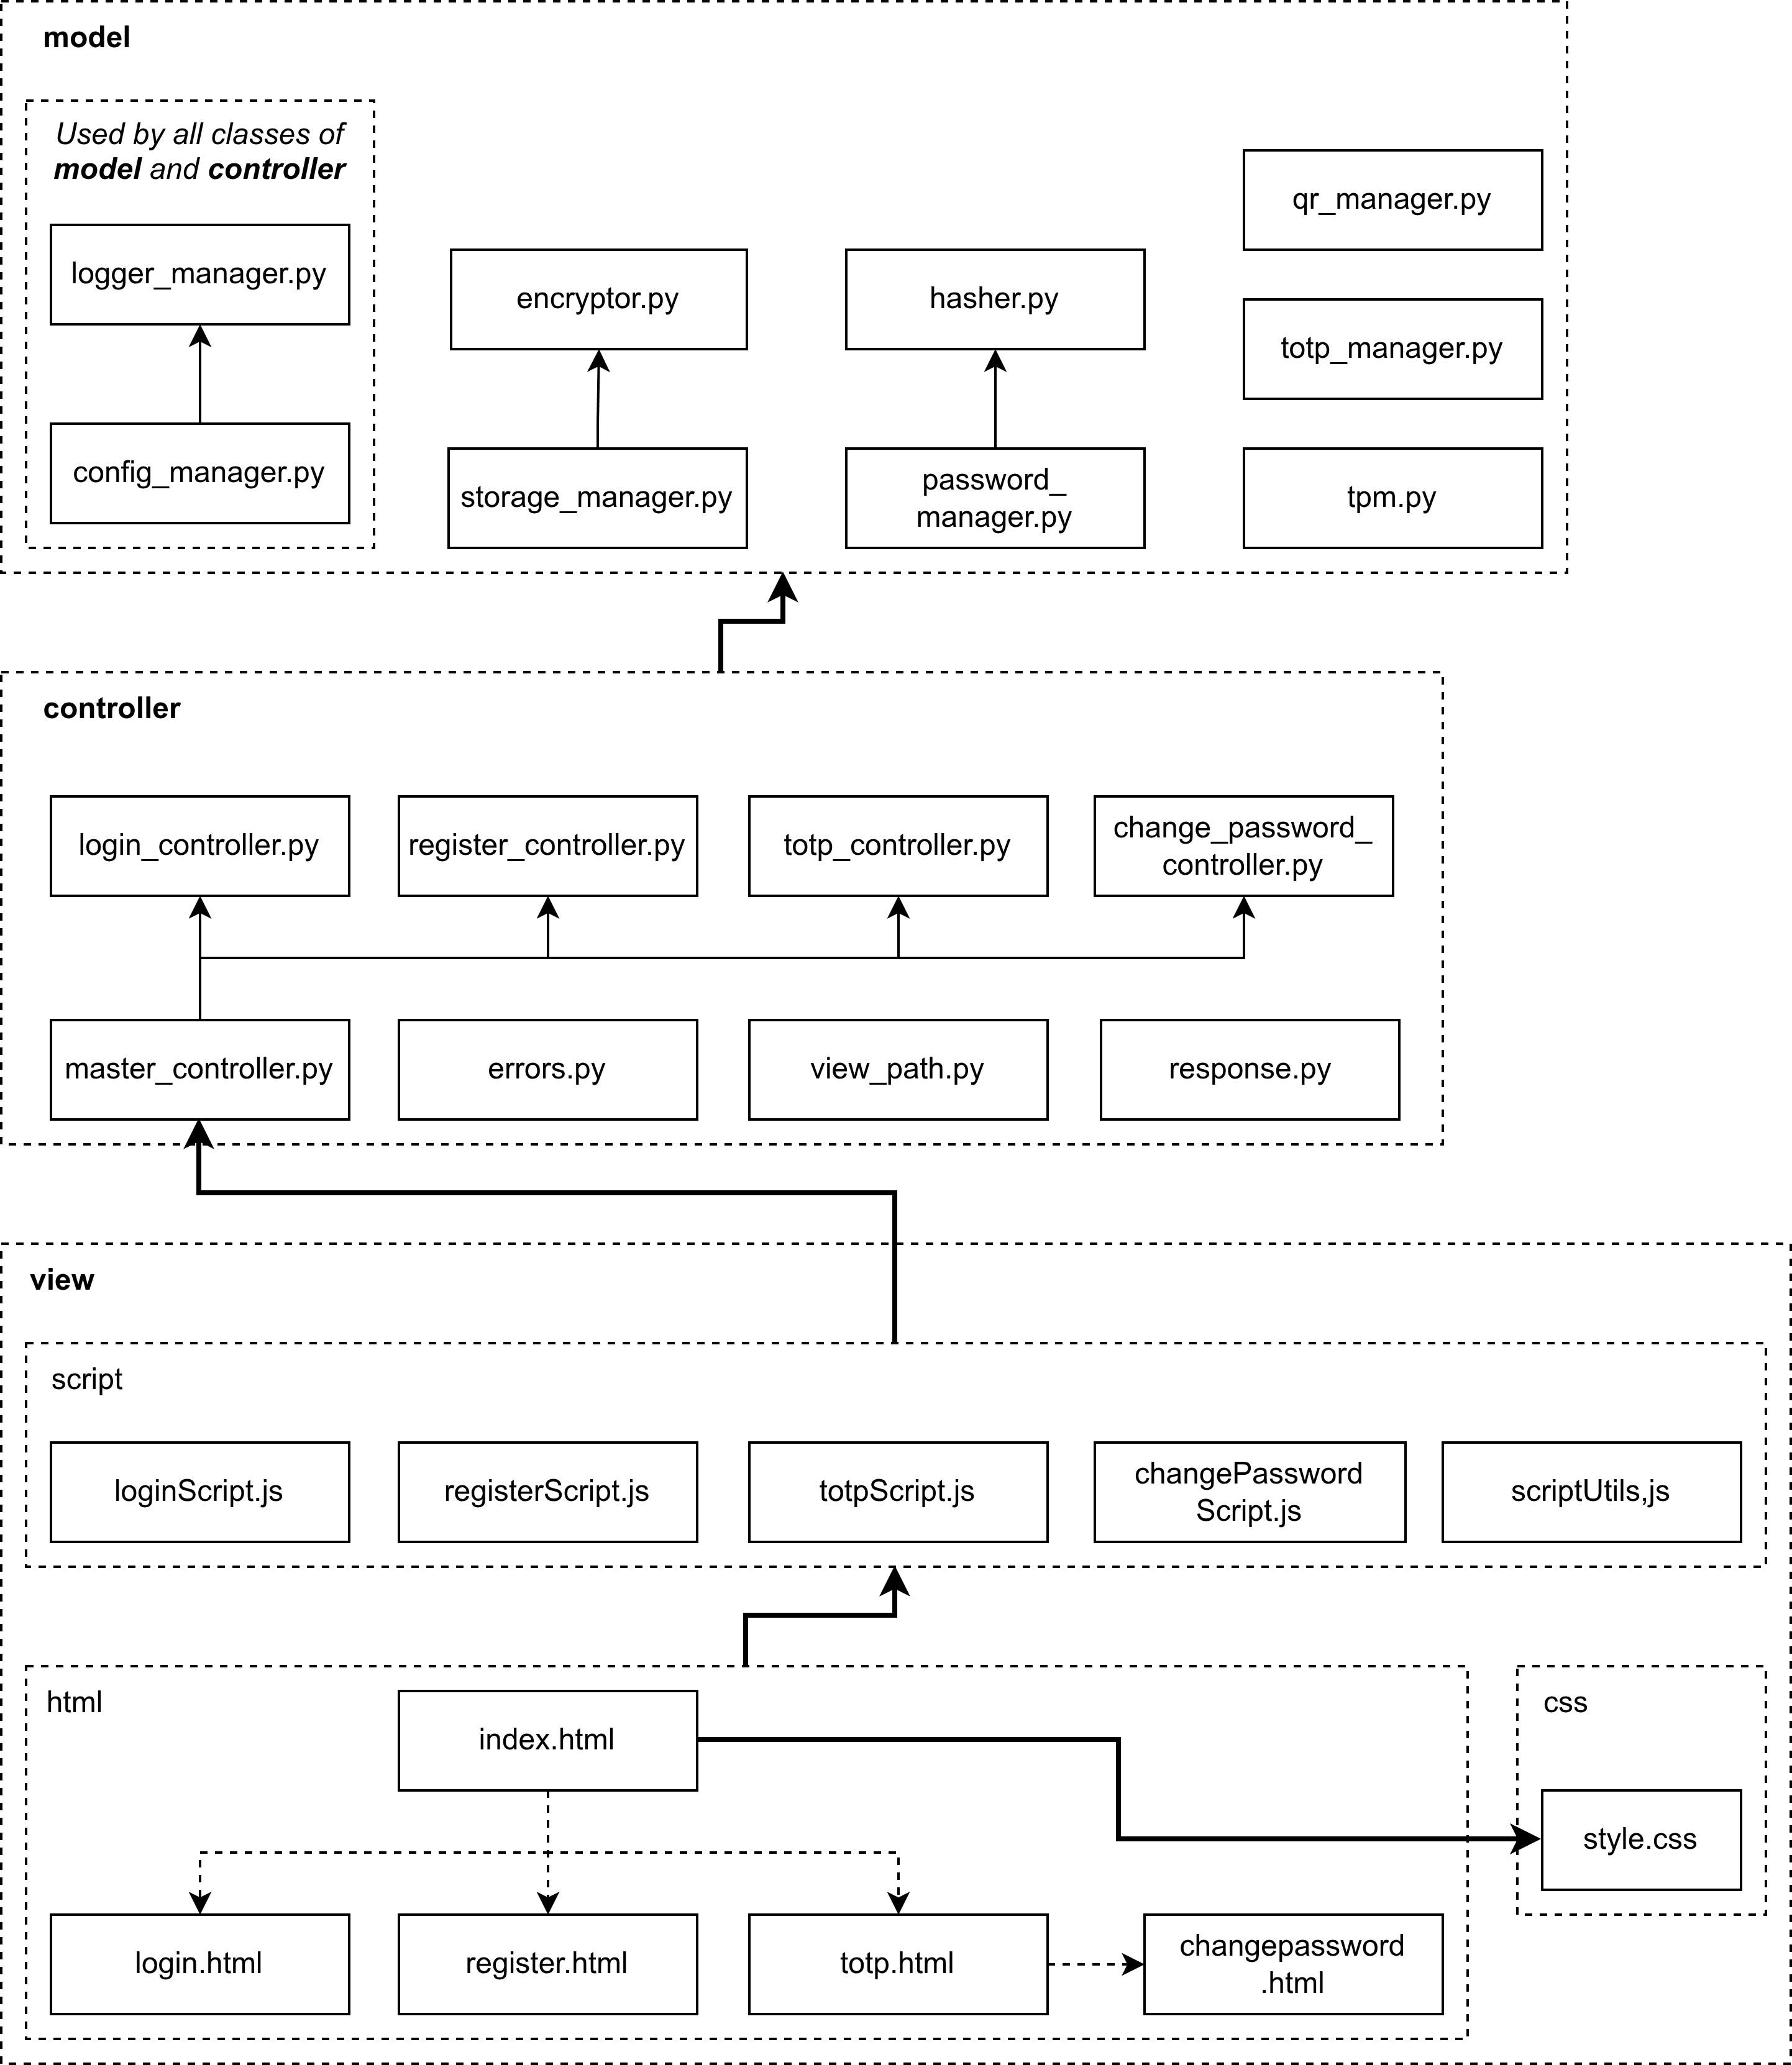
\includegraphics[width=\textwidth]{img/diagram-high-level.png}
    \caption{High-level diagram of \app{}.}
    \label{fig:high-level}
\end{figure}

\app{} uses the \t{pywebview} library to provide a desktop application GUI which is written in web technologies.
I chose to write HTML and CSS instead of using native GUI elements for a more uniform and cross-compatible experience.
I kept design simple, without going too heavy on JavaScript.
There are no JS libraries or frameworks included, since that would have a huge impact on the project size and performance.
Keep in mind that \app{} needs to run on a USB stick, so choosing lightweight solutions is a must.

Each of the packages will be described in detail in the following.
When thinking of flows, or when interpreting Figure \ref{fig:high-level}, keep in mind that everything is triggered by the actions of the user.
Flow always starts from view, where JS triggered by either the user interacting with HTML elements or by periodic method calls/ timers.
Then, the JS handler methods delegate to controller handler methods, which orchestrate the classes of model, calling business functionalities and tying them together.
The model classes are kept as independent as possible, and they are unit tested.

\subsection{Model} \label{lab:ch4-model}

As mentioned earlier, the back-end of the application is written in Python.
While it might sound like a weird choice for a security-first application, there are reasons for this decision.
First and foremost, Python provides a lot of libraries, making implementation easier.
Using standard implementations and not reinventing the wheel is usually the better approach for small teams.
This is even more true if we talk about cryptographic algorithms, like encryption and hashing.
\app{}'s backend contains plenty of these, so developing in Python enabled access to a lot of standard, popular, community-audited libraries.

Second of all, Python provides an easy way to manage dependencies.
When implementing \app{}, I also focused on making the developer experience easier.
The setup of a project is always a big pain in the butt; Python's package manager (\t{pip}) makes it bearable.
All the libraries are downloaded inside a virtual environment (\t{venv}), so they are isolated and do not mess with the system's packages.
The downloaded packages are then listed inside a \t{requirements.txt} file, so one can install all of them with a single command.

While Python isn't famous about its OOP capabilities, I chose an object-oriented approach.
For me and for most developers, it is simply a thing of habit to think of complex problems in terms of classes, objects, and interactions between objects.
It provides structure and a common language.
In \app{}, (almost) every Python file contains exactly one class, kind of like how Java enforces it.
Interfaces are implemented using \t{ABC} and \t{abstractmethod} from the \t{abc} library.
The overridden methods are marked with the annotation \t{override} from the \t{typing\_extensions} library.
These mechanisms do not cause runtime errors, but generate warnings in the right IDE, making it easier to catch bugs.

Similarly, the \t{typing} library is used for type hinting.
Python is duck-typed, meaning that for Python, if something quacks, it is a duck.
``The Python runtime does not enforce function and variable type annotations.''\footnote{\url{https://docs.python.org/3/library/typing.html}}, but the \t{typing} library provides runtime support for type hints.
The data type of method parameters and the return values of the methods can be specified. 
Mismatches will generate warnings.
Type hints also document intent: it is easier to understand what the method tries to achieve if you can picture the underlying data types.

The backend consists of several packages, which will be presented in the following sections.
Each package is self-contained, i.e., independent of the other.
As a result, they can be (and are) unit tested (see: Section \ref{ch5-theoretical-and-experimental-results}).
As a secondary side-effect, this isolation made it so that for most classes it made sense to use the Singleton pattern.
The singleton pattern ensures that there is just one instance of a given class at a time.


\subsubsection{Singletons, singletons everywhere.} \label{lab:ch4-singleton}

Since I wanted easily manageable classes, and probably since I am influenced by the fact that I worked with Java Beans for the last couple of months, all the classes of model follow the singleton pattern.
The main reason is philosophy: these classes encapsulate logic and state which shall be the same over the whole application.
Encryption, hashing, TOTP code generation etc. all work the same way, independently of where they will be called.
In some cases, static methods would have been enough, but for uniformity, and since static is not always an option, everything is a singleton class.

An example where singleton makes life easier than a pure static design: encryption.
While \app{} never stores the user password and the salt on disk, they are kept as class fields of singleton \t{Encryptor}.
Yes, this means the secret is stored in RAM, but so it is if it's just read for a split second.
Having it as class fields, we do not need to re-prompt the user at each encryption operation, nor to query the TPM for the secret each time.

There are two types of singletons in \app{}.
The classes with ``Manager'' in their name are simple singletons, for example, \t{LoggerManager}.
It contains a \t{instance} field.
If the constructor is called and \t{instance} is not None, it is returned instead of running a new initialization.
Else, \t{instance} is built up by filling its fields, running initialization logic and everything that happens in a constructor, as usual.
The seconds type of singletons define a facade for multiple classes.
For example, \t{TPM} is the TPM singleton: it has the usual singleton logic, but it also picks the right TPM class from a pool of multiple possibilities depending on the platform and the configs.
Each option implements \t{AbstractTPM}, which is the common interface.
This pattern is used where flexibility is desired: we want a singleton, but we have options for the specific class.


\subsubsection{Configurations and how \app{} is made parametrized.} \label{lab:ch4-config}

\app{} has certain parameters which can be changed from a JSON file, without changing source code.
The \t{config} package contains the \t{ConfigManager}, as well as one or two JSON files.
The \t{ConfigManager} is a singleton class, used by all of the classes of the model and controller.
It exposes a method, through which a JSON configuration file is parsed, and the config requested as a parameter is returned.
This way, the user of the application can change the behavior of \app{} without downloading a new release or changing the source code.

The name of the config file is hardcoded, and it is \t{config.json}.
It has multiple levels, as show in Listing \ref{lst:config-json}.
Developers also have the possibility to define a \t{config-local.json} file, which, if present, has priority over \t{config.json}.
The local config file shall be in \t{.gitignore} and used solely for local development.

\begin{lstlisting}[language=JSON, label={lst:config-json}, caption={An example configuration file.}]
{
  "logger": {
    "log_level": "DEBUG",
    "log_file_path": "log.txt"
  },
  "encryptor": {
    "type": "AES"
  },
  "hasher": {
    "type": "ARGON2"
  },
  "password": {
    "min_length": 15,
    "max_length": 100,
    "hash_file_path": "hash.txt"
  },
  "storage": {
    "storage_file_path": "storage.txt"
  },
  "pywebview": {
    "debug": false,
    "width": 450,
    "height": 800
  },
  "tpm": {
    "enabled": false,
    "virtual": {
      "fapi_profile": "P_RSA2048SHA256",
      "fapi_profile_url": "https://raw.githubusercontent.com/tpm2-software/tpm2-tss/3.2.0/dist/fapi-profiles/P_RSA2048SHA256.json",
      "enabled": false,
      "tpm_path": "/tmp/vtpm",
      "tpm_port": 2321,
      "tpm_ctrl_port": 2322,
      "tpm_start_wait_s": 1
    }
  }
}
\end{lstlisting}

The meaning of each parameter is the following:
\begin{itemize}
  \item \t{logger.log\_level}:
    The log level to use for the one and only logger.
    Everything higher or equal will be logged, everything lower will be ignored.
    Accepted options: \t{DEBUG}, \t{INFO}, \t{WARNING} \t{ERROR}.
  \item \t{{logger.log\_file\_path}}:
    The path of the log file.
    Logs are written to console but also to a log file, for audit, troubleshooting, and for cases there a console is not available.
  \item \t{encryptor.type}:
    The encryptor to use.
    As of v1, only \t{AES} is supported.
  \item \t{hasher.type}:
    The hasher to use.
    As of v1, only \t{ARGON2} is supported.
  \item \t{password.min\_length}:
    The minimum length required for user password, inclusive.
  \item \t{password.max\_length}:
    The maximum length accepted for user password, inclusive.
  \item \t{password.hash\_file\_path}:
    The path to the hashed user password file. 
  \item \t{storage.storage\_file\_path}:
    The path to the storage file.
  \item \t{pywebview.debug}:
    If set, pywebview's debug mode is enabled.
    Accepted options: \t{True}, \t{False}.
  \item \t{pywebview.width}:
    The width of the pywebview window.
  \item \t{pywebview.height}:
    The height of the pywebview window.
  \item \t{tpm.enabled}:
    If set, TPM functionalities are enabled.
    Accepted options: \t{True}, \t{False}.
  \item \t{tpm.virtual.fapi\_profile}:
    Which FAPI profile to use for the virtual TPM.
    Will be passed to \t{fapi-config.json}, and used as file name for the FAPI profile file.
    Must be in sync with parameter \t{tpm.virtual.fapi\_profile\_url}.
  \item \t{tpm.virtual.fapi\_profile\_url}:
    The URL from which the FAPI profile can be downloaded for the virtual TPM.
    Must be in sync with parameter \t{tpm.virtual.fapi\_profile}.
  \item \t{tpm.virtual.enabled}:
    If set, the software TPM is used instead the real TPM chip.
    Setup will run based on other \t{tpm.virtual} parameters.
    Accepted options: \t{True}, \t{False}.
  \item \t{tpm.virtual.tpm\_path}:
    Since TPMs on Linux are device nodes, this is the path to use for the virtual TPM.
  \item \t{tpm.virtual.tpm\_port}:
    The port to use for the virtual TPM.
  \item \t{tpm.virtual.tpm\_ctrl\_port}:
    The control port to use for the virtual TPM.
  \item \t{tpm\_start\_wait\_s}:
    The amount of seconds to wait before checking if the virtual TPM got successfully provisioned, after calling the provision function.
\end{itemize}


\subsubsection{How logging is done.}

Logging is done by the package \t{Logger}.
It contains the \t{LoggerManager} class, yet another singleton.
As its name suggests, the logger manager provides a logger instance.
It is the one and only way to print messages, the print statement and similar shall not be used.

The standard \t{logging} library is used.
The log level can be from config (see: Section \ref{lab:ch4-config}).
For simplicity, \app{} uses only four log levels.
It is important to select the right log level each time, otherwise important logs might get cluttered or not printed with certain configs.
From most severe to the least, these are:
\begin{enumerate}
    \item \b{Error}. For fatal issues, ones which break execution.
    \item \b{Warning}. For issues which should not be ignored, but do not crash the app.
    \item \b{Info}. For messages which are not issues, but things that might help in audit.
    \item \b{Debug}. The most low-level messages. These are useful only for development.
\end{enumerate}

While the logger is centralized, logging happens in two places: the console and the log file.
The same log lines are printed in both outputs, but the log file persists, meaning that new logs are appended to the old ones instead of starting a new file at each run.
This is helpful for debugging and provides a possibility to audit previous actions, for example, if someone else tried to log in.

The format of log lines is: date and time, severity level in a letter (E, W, I, D), the file and the line of the source, the logger, and the message itself.
Some log lines are shown on Figure \ref{fig:log-example}.
While there is only one logger instance, \t{pywebview}, the front-end library also logs its warnings and errors.
These are useful, so instead of throwing them out, they are ``propagated'' to \t{LoggerManager}'s instance.
This is why the logger is also printed in the log line: it can be either \t{[root]} or \t{[pywebview]}.

\begin{figure}[htbp]
    \centering
    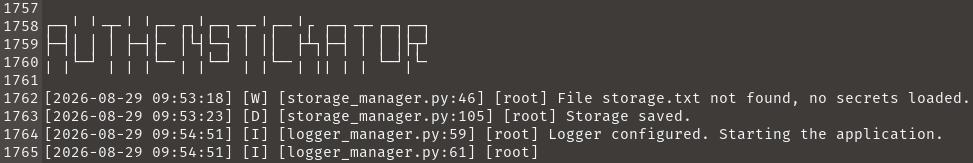
\includegraphics[width=\textwidth]{img/log-example.jpeg}
    \caption{Example log lines from the log file.}
    \label{fig:log-example}
\end{figure}

As a general rule, secrets and sensitive data shall never be logged.
Logging such information be the equivalent of a data leak.


\subsubsection{Generating TOTP codes.} \label{lab:ch4-totp}

Class \t{TOTPManager} is responsible for generating the TOTP codes, as well as other TOTP-related functionalities.
The \t{pyotp} library was used, which is straight-forward and provided every functionality I needed.
As a matter of fact, there are only two such functionalities: generating TOTP-related information and parsing TOTP URIs.

By \b{TOTP-related information}, I mean the current six-digit code, the next six-digit code, when the current code expires, and when the next code expires, as well as the interval.
The \b{interval} is the time for which one TOTP code is valid.
It is usually set to 30 seconds, as recommended by the authors of the TOTP algorithm.\cite{totp}
However, \app{} does not assume it is 30 seconds all the time, instead it deduces it from the secret.
Deducing the info from the secret is as simple as calling a constructor and then extracting its fields, although some mathematics had to be done.

Counterintuitively, I do not send to the frontend the seconds remaining.
This would be a huge overhead, just think about it: querying every second for every secret, just to get back the same redundant information roughly 58 times a minute.
Instead of querying each second, I could just automatically send each second, but again, this is a lot of redundancy, and it does get hacky.
Instead, what I chose to do, is to send the expiration times to frontend, and let the frontend calculate the remaining time.
Some kind of loop/ repetitive check is needed anyway, and a frontend timer is probably the best solution.
The frontend can then query for fresh information when the current code expires.

But what happens, if the querying takes longer than expected?
Or if the number of codes to query for is large, and they expire at the same time, causing an unexpected overhead?
Actually, the latter is rather expected, as almost all apps use the default TOTP parameters, and hence their codes all expire at the same moment (I have not seen any counter-examples yet).
Well, this is why I also send the next code.
It is trivial, and the TOTP algorithms allows us, to retrieve the next code.
In fact, any code could be computed, since the code is a function of the current time.
There are authenticator apps, like Proton Authenticator, which also show the next code.
So, the frontend has the current code and also the next one: when the current code expires, it can instantly \b{promote} the next code, i.e., make it current.
This results in a smooth transition.

\b{Parsing the TOTP URI} means extracting information from the URI which the apps usually show in QR form.
Yes, those fancy QR codes are nothing more than just a ``link'', which usually/hopefully follows the Key Uri Format specified by Google\footnote{\url{https://github.com/google/google-authenticator/wiki/Key-Uri-Format}}.
In the \t{TestTOTP} test class you can see some examples of such URIs, as different platforms provided to me:

\begin{enumerate}
  \item \url{otpauth://totp/totp@authenticationtest.com?secret=I65VU7K5ZQL7WB4E}
  \item \url{otpauth://totp/Google\%3Arolandtest123456\%40gmail.com?secret=refyopv7thgvsd5twr3marvdpqyugxls\&issuer=Google}
  \item \url{otpauth://totp/Microsoft:rolandtest123456@gmail.com?secret=G5HLROANXBF7335S\&issuer=Microsoft}
\end{enumerate}

The first one comes from the test site \url{https://authenticationtest.com/totpChallenge/}, which I used a lot throughout development.
It provides a hardcoded secret, both in plaintext and in QR form.
The QR, when parsed, resulted the URI shown with number 1.
Comparing it with the Key Uri Format examples, you can see that it contains the label \t{totp@authenticationtest.com}, and the secret \t{I65VU7K5ZQL7WB4E}.
It does not contain the issuer, although it is ``STRONGLY RECOMMENDED'' by Google, it is not required, hence we cannot assume that we get it all the time.
The second URI comes from a dummy Google account I made.
You can see that it used URL encoding\footnote{\url{https://www.calculator.net/url-encode-decode.html}}: \url{\%3A} $\rightarrow$ \t{:}, \url{\%40} $\rightarrow$ \t{@}.
The label also contains the issuer.
The third URI is from a dummy Microsoft account.
Similarly to number 2, this one also specifies an issuer, and the label already contains the issuer.

In \app{}, storage contains just two information: the secret and the name.
The name is combined as \t{ISSUER:LABEL}, if both available, or just the label, if it already contains the issuer, or just label, if issuer is not provided.


\subsubsection{Decoding QR images.}

Every mobile authenticator app provides the possibility to scan the QR code provided by the app which requires MFA.
But, a USB stick does not have a camera.
Initially, the only way to enter a TOTP secret into \app's database was to enter the secret manually, enter a name manually, and press enter.
But, what if the app only shows a QR, and does not give us the plaintext equivalent?
In that case, we could use an online tool to decode the QR image, but this would mean that we blindly trust a random website with handling out sensitive information.

As a solution, I integrated QR decoding functionality into \app{}.
It requires an image of the QR code, so a snip has to be saved beforehand.
\b{The user shall delete the screenshot after decoding it, or store it in a secure location.}
Otherwise, the secret could be exposed.
The app could delete the image after decoding, but it leaves it to the user; who am I to manipulate your files?
It would kind of break the isolation idea of \app{}, according to which the territory of \app{} is only the USB stick.

The QR code image is decoded using the \t{zxingcpp} library.
Initially, \t{pyzbar} was used, but it brought extra requirements for Windows packs, so I switched it to \t{zxingcpp}, which is newer and still maintained.
With the \t{pillow} library I opened the image, and with the \t{zxingcpp.read\_barcodes(image)} call I got the decoded text.
The text is a URI which is passed to TOTP for parsing (see: Section \ref{lab:ch4-totp}).
If there are no QR codes found in the image, I return None.
If there are multiple QR codes, the first one is processed, and a warning is logged.


\subsubsection{Hashing and checking against a previous hash.} \label{lab:ch4-hasher}

\app{} currently uses the Argon2 algorithm (see: Section \ref{lab:ch3-argon2}) in its \t{Argon2Hasher} class for hashing purposes.
The \t{argon2-cffi} library is used.
It provides a hashing and a verifying method.
It is worth noting that the same input creates different hashes, so verification is a library function call as well, not hashing and a simple equals operation.
The latter would not give correct results.


\subsubsection{Policies for the user password.}

The \t{PasswordManager} class implements the password policies for \app{}.
It is generally a good practice to extract password management into a separate class or module, to apply the same rules everywhere.
This is the only class which uses the user password hash file, no other classes shall read from or write to it, or modify it in any way.
The class exposes a method for checking if a previous password was provided, which does nothing more than check if the user password hash file exists.
This method determines upon startup if we go through the register or through the login scenario.

The password manager is also responsible for validating new passwords.
If they satisfy complexity requirements, it is said that they are ``acceptable''.
An acceptable password in \app{} has a length between a minimum and a maximum length specified by configs (see: Section \ref{lab:ch4-config}).
But, since \app{} takes security seriously, if the minimum length parameter is set to less than 15, it is switched to 15.
This is to follow the guidelines published by NIST SP 800-63B-4\footnote{\url{https://nvlpubs.nist.gov/nistpubs/SpecialPublications/NIST.SP.800-63B-4.pdf}}, Section 3.1.1, which says:
``Verifiers and CSPs SHALL require passwords that are used as a single-factor authentication mechanism to be a minimum of 15 characters in length.''

There is no special character requirement and such craziness.
We are well past the age where special characters provided any benefit.
Nowadays, they are rather an obstacle, in defining long a memorable passphrase.
The same NIST article, in its Appendix called Strength of Passwords, doubles down on this idea, saying that:
\begin{itemize}
  \item
    ``Password length is a primary factor in characterizing password strength''
  \item
    ``Research has shown that users respond in very predictable ways to the requirements imposed by composition rules.
    For example, a user who might have chosen “password” as their password would be relatively likely to choose “Password1” if required to include an uppercase letter and a number or “Password1!” if a symbol is also required.''
  \item
    ``Other mitigations (e.g., blocklists, secure hashed storage, machine-generated random passwords, rate limiting) are more effective at preventing modern brute-force attacks, so no additional password requirements are imposed.''
\end{itemize}

The password manager uses the hasher (see: Section \ref{lab:ch4-hasher}) to hash the user password before saving it to the user password hash file, and to verify the correctness of a provided user password, by reading the hash and verifying against it.
Setting a new password implicitly involves checking if the new password is acceptable.
There is also a hard limit of 100 maximum characters for the password, but this is just a sanity check, to avoid crazy users causing an overflow.


\subsubsection{TPM and the generation of the TPM secret.} \label{lab:ch4-tpm}

\app{} currently supports TPM functionalities only on Linux (see: Section \ref{lab:c6-further-improvements}).
Using the second singleton approach described in Section \ref{lab:ch4-singleton}, the \t{TPM} class chooses between \t{NoTPM}, \t{LinuxTPM} and \t{WinowsTPM}, where \t{WindowsTPM} contains identical implementation to \t{NoTPM}.
If TPM functionalities are disabled from configs (see: Section \ref{lab:ch4-config}), \t{NoTPM} is chosen.
Otherwise, the current platform dictates what to do.
\t{LinuxTPM} also provides support and setup for a virtual TPM, for development purposes.

As explained in \cite{pi3g_tpm_2025}, on Linux, TPM shows up as device nodes.
\t{/dev/tmp0} is the Hardware Interface, while \t{/dev/tpmtm0} is the Kernel Resource Manager.
Most applications use the Kernel Resource Manager, since through that entry the kernel handles context management and other low-level mechanisms.

TSS stands for Trusted Software Stack, and it is the software around the TPM chip.
It has a layered architecture, providing programmer-friendly API calls.
Its layers are specifications, and there are different implementations of it.
The four layers are:

\begin{enumerate}
    \item \textbf{FAPI}: Feature API. High-level, developer-friendly. No need to handle sessions and authorization.

    \item \textbf{ESAPI}: Enhanced System API. Wraps sessions and handles retries when TPM is busy.

    \item \textbf{SAPI}: System API. Low-level C interface implementing the tmp2.0 specifications.

    \item \textbf{TCTI}: TPM Command Transmission Interface. The Transport Layer, working with bytes.
\end{enumerate}

\app{} uses the \t{tpm2\_pytss} library and the FAPI layer.
FAPI was chosen since it is the most high-level, so the resulting code will be more generic.
Going lower in the TSS layers would mean more OS/ hardware specific code, and more chances to make errors.

When this layer is used, configurations are held in a file named \t{fapi-config.json}.
The default location is \t{/etc/tpm2-tss/fapi-config.json}, but it can be overwritten by setting the \t{TSS2\_FAPICONF} environment variable.
This file is generated automatically when you install or compile the libraries for FAPI provisioning, and it looks as shown in Listing \ref{default-fapi-config}.
\b{Provisioning} is an initialization step necessary to be performed before using FAPI.
The TPM, FAPI and the related files and configs are not well documented, so most of what I write here are the results of trial and error.

\begin{lstlisting}[language=json, label={default-fapi-config}, caption={The default FAPI configuration file, as on my system.}]
{
  "profile_name": "P_ECCP256SHA256",
  "profile_dir": "/etc/tpm2-tss/fapi-profiles/",
  "user_dir": "~/.local/share/tpm2-tss/user/keystore",
  "system_dir": "/var/lib/tpm2-tss/system/keystore",
  "tcti": "",
  "system_pcrs": [],
  "log_dir": "/var/run/tpm2-tss/eventlog/",
  "firmware_log_file": "/sys/kernel/security/tpm0/binary_bios_measurements",
  "ima_log_file": "/sys/kernel/security/ima/binary_runtime_measurements",
  "ek_cert_less": "yes"
}
\end{lstlisting}

Provisioning a real TPM might require authorization, or might have been done beforehand is there is other software using FAPI.
This is a tedious task which might differ from hardware to hardware, includes many edge cases and possible error sources.
I generated with the help of AI a setup script for provisioning, which worked on a fresh Ubuntu 22.04 installation, see Section \ref{lab:ch4-provisioning-the-tpm-on-linux}.
You can try it, or do it manually, but note that a provisioned FAPI is a prerequisite if you select non-virtualized TPM from configs.

For development, but strictly only for that, a virtual TPM is encouraged, which can be opted for through the configs.
By using a virtual TPM, you won't get locked out of the real TPM if you repeatedly violate authorization.
A virtual TPM can be wiped completely anytime, and a new instance can be started.
For the virtualization of the TPM, the \t{swtpm} Linux library is used.
The \t{LinuxTPM} class contains code for setup which should work out of the box, running each time if you selected virtualization.
It creates a custom \t{fapi-config.json}, as seen in Listing \ref{virtual-fapi-config}.

\begin{lstlisting}[language=json, label={virtual-fapi-config}, caption={The virtual FAPI configuration file, as on my system}]
{
    "profile_name": "P_RSA2048SHA256",
    "profile_dir": "/home/broland/.local/share/authenstickator/profile-dir",
    "user_dir": "/home/broland/.local/share/authenstickator/user-dir",
    "system_dir": "/home/broland/.local/share/authenstickator/system-dir",
    "tcti": "swtpm:port=2321",
    "system_pcrs": [],
    "log_dir": "/home/broland/.local/share/authenstickator",
    "ek_cert_less": "yes"
}
\end{lstlisting}

You can note the slight differences: there is a port defined, and a different profile is used.
The FAPI profile is downloaded from the internet, from the URL specified in the config file.
The profile's version shall match the version of the installed native \t{tpm2-tss/libtss2-fapi}.
This can be retrieved with the help of the command \t{apt policy libtss2-fapi1}.
Note that this is different from the \t{tpm2-pytss} version shown in \t{requirements.txt}.

If configuration, provisioning, and all the setup steps are done correctly and successfully, the actual usage of the TPM through FAPI reduces to just a few lines.
These high-level functions provide convenient wrappers for TPM functionalities.
The random number (TPM secret) is generated with \t{fapi.get\_random(16)}, where 16 means the secret will be of 16 bytes length.
This number is then saved to and later retrieved from the TPM's Non-Volatile Random Access Memory (NVRAM), using the \t{fapi.create\_nv}, \t{fapi.nv\_write} and \t{fapi.nv\_read}.
For each method, I used the same path, which basically defined the slot of NVRAM used, but abstracted, without going to index and byte level.
The existence of the TPM secret before generation is checked with \t{fapi.list("/")}, which gets a list of all FAPI object paths.
If the result contains our path, it means the secret was generated.

The FAPI method \t{create\_nv} is called with the flag \t{exists\_ok=True}, and \t{provision} (for the virtual TPM) is called with flag \t{is\_provisioned\_ok=True}.
Both of these, in the case of previous create/provisioning, write an error in the log files, but do not actually cause crash.
This is because \t{tpm2-pytss} is a wrapper for the \t{tpm2-tss} library written in C, and this is the best the wrapper's authors could come up, I guess.
This is a beauty flaw of the logs, but they do not mean actual errors.


\subsubsection{Encryption and decryption.} \label{lab:ch4-encryptor}

While the encryptor singleton allows the existence of multiple encryptors, currently only \t{AESEncryptor} is implemented.
As its name suggests, it uses the AES algorithm (see: Section \ref{lab:ch3-aes}).
The user password and the TPM secret is run through the PBKDF2 algorithm (see: Section \ref{lab:ch3-pbkdf2}).
This basically combines the user password, which could be of any length (between the limits imposed by the configs), and the TPM secret, which is used as salt, into a key of 32 bytes length.
The result can be used as a key for the AES algorithm.
AES is a symmetric algorithm, so the same key is used for encryption and decryption.

The libraries \t{Crypto.Cipher}, \t{Crypto.Hash} and \t{Crypto.Protocol.KDF} are used for \t{AES}, \t{SHA256} and \t{PBKDF2}, respectively.
For the PBKDF2 algorithm, I used 600000 iterations, with SHA256, as specified by the OWASP Password Storage Cheat Sheet\footnote{\url{https://cheatsheetseries.owasp.org/cheatsheets/Password_Storage_Cheat_Sheet.html\#pbkdf2}}.
This is a work factor, and having a high value means it is harder to brute-force, but slower for malign use as well (it is ``intentional slowness'').
So instead of balancing between security and usability with random trial and error, I consider that following trusted guidelines is a better option.

This AES library works with triplets of nonce, tag and ciphertext, i.e., the AES-EAX variant of the algorithm.
In practice, this means that at each encryption I create a new cipher using \t{AES.new}.
The ciphertext returned by the \t{AESEncryptor}'s \t{encrypt} method will then contain the nonce, concatenated with the tag and the actual ciphertext.
At decryption, this triplet is split.
A new cipher is created with the same key and the extracted nonce, and the tag is passed to \t{decrypt\_and\_verify} to ensure correctness.
This approach avoids the common pitfall of using the same nonce twice, which often turns such algorithms ``from gold-standard to broken'' (see \footnote{\url{https://www.trustedcalcs.com/en-us/guides/dev-tools/aes-gcm-encryption}} for an article which describes AES-GCM, which is another variant but at high level api point of view works the same way).

The \t{AESEncryptor} and its respective singleton class, \t{Encryptor}, went through multiple refactorings throughout development.
The final version does not set the key in the \t{\_\_init\_\_} method, but has a dedicated \t{set\_key} method.
This is because the user password can change: \app{} supports password reset.
In such cases, we want to change the key, but we do not want to swap out the singleton instance.
The \t{set\_key} solves this exact issue: the key (internal state) is changed, but the instance (the reference) remains the same, so the change is ``implicitly propagated'' throughout the code base.


\subsubsection{How the storage file is handled.}

The \t{StorageManager} class is the one responsible for handling storage.
Storage means the ``database'', which in practice is a single file, called the storage file.
The storage file's path can be defined as a config (see: Section \ref{lab:ch4-config}).
Storage manager uses the encryptor (see: Section \ref{lab:ch4-encryptor}) to decrypt the storage file upon initialization.
If encryption fails (either the key is wrong, although password checking should guard against this, or the file is broken, against which \app{} cannot protect), storage initialization is considered failed, and the \t{\_\_new\_\_} method returns None.
This has to be handled by the caller.

After successful decryption of the storage, the result is a JSON file which maps to a one-layer dict, where the key is the name (as described in Section \ref{lab:ch4-totp}), and the value is the TOTP secret.
The choice is intentional and would not work in reverse: the secret is provided by the user once, after which the UI only holds reference to the name, hence queries by name.
Keeping the secret in the UI would mean an information leak.
The fact that the underlying data structure is so simple makes saving trivial, symmetric to retrieval: the internal storage is dumped (\t{json.dumps}), the dump is encrypted, and the ciphertext is written to the file.

The class exposes methods for adding a secret, removing a secret, getting a secret.
There is also a ``get all secrets'' method, which shall be used at startup to load all the data.
These methods have straight-forward validations: an entry cannot be added if the name is already in use, an entry cannot be removed and/or retrieved if it does not exist.

Initially, I wrote the \t{StorageManager} to support the Context Manager Protocol, i.e., such that it can be used with Python's \t{with} syntax.
This meant that \t{StorageManager} was used inside a \t{with} block, and when execution got out of it in any form (the instructions were all executed or an exception happened), a cleanup function was called.
However, I found an even stronger and more robust solution: just save each time we modify storage.
This leaves no space (as in time window of intermediary instructions) for things to mess with storage.
If a secret is successfully added, the file is saved.
If a secret is successfully deleted, the file is saved.
This might sound like a huge overhead, but it is not: adding and removing secrets is not a frequent operation.
And, let's be real, how many TOTP secrets can a user have at most?






\subsection{View} \label{lab:ch4-view}

\subsection{Controller} \label{lab:ch4-controller}





\section{Development} \label{lab:ch4-development}

\app{} was developed on a relatively old laptop running Pop!\_OS 22.04 LTS.
For source control, just like every sane developer, I used Git.
The project is available as a public GitHub repository at \url{https://github.com/broland29/authenstickator}.
It has GPL-3.0 license, meaning it can be used freely as long as the product which uses is also open source.

The IDE used for development was PyCharm 2026.1.4.
The default Python formatter was used (Settings $\rightarrow$ Editor $\rightarrow$ Code Style $\rightarrow$ Scheme: Default), with a hard wrap at 100 columns.
100 characters is reasonable for Python code, for JS, HTML and CSS I did not set such limits.
I also set to format the code on each save (Settings $\rightarrow$ Actions on Save $\rightarrow$ tick Reformat code and Optimize imports).

The documentation was written in Latex, using Visual Studio Code 1.128.0 and the LaTeX Workshop extension.
For spell checking, the LTeX+ extension was used, which is completely offline.
The source code of the documentation is also under version control, available at \url{https://github.com/broland29/authenstickator-docs}, under the same license.
The starting point of the documentation was the template provided by the Technical University of Cluj-Napoca, available at \url{https://cs.utcluj.ro/studii-de-masterat/sesiunea-ii-septembrie-2026.html}.



\subsection{Dependency Management, Imports} \label{lab:ch4-dependency-management-imports}

For installing packages and keeping track of their versions, \t{pip} was used.
Some packages installed through \t{pip} also have OS-related dependencies, which will be discussed in later sections.
But, in principle, \t{pip} was the one and only source of packages.
Then, a \t{requirements.txt} file was generated using pip freeze.

\begin{lstlisting}[language=bash, label={lst:pip-freeze}, caption={Generating the requirements file.}]
pip freeze > requirements.txt
\end{lstlisting}

This file contains all the packages and their versions.
Even though \app{} was developed with cross-platform portability in mind, some functionalities, like the usage of TPM, required platform-specific packages.
These are also marked in the requirements file, like: \t{sys\_platform == "linux"}.
If, during development, new dependencies are added, or versions are updated, the command \ref{lst:pip-freeze} has to be run again.
But, be careful with updating packages: while I tried bringing everything to the latest version, there are some packages which simply do not work with newer versions, like \t{PyGObject}.

Dependencies are not installed directly on the whole system, but a virtual environment is used.
A virtual environment (\t{venv}) is used to isolate Python packages used for \app{} from other Python packages on the system.
This is standard dependency management, and ensures not just that \app{} works well, but that we don't break other apps.
Each developer creates its own virtual environment and these are not pushed to git (specified in \t{.gitignore}).

The application is run as a module (with the \t{-m} flag).
It is important to have every import start from the \t{src} folder.
Even if relative imports work in PyCharm (due to hacks PyCharm does in the background), not following this convention will have nasty side effects: running from the CLI with the usual command will simply not work.
The same convention has to be kept in tests also, since I hit unwanted side effects due to importing files differently in tests than in source code.
Make sure to set \t{authenstickator} as a Source Root (see: \footnote{\url{https://stackoverflow.com/questions/52949551/is-there-any-way-to-force-pycharm-to-always-use-absolute-imports}}).



\subsection{Setup and Packing}
\app{} is meant to run on a USB Stick, on machines which possibly do not even have Python.
One such release candidate is made with the help of PyInstaller.
``PyInstaller bundles a Python application and all its dependencies into a single package.
The user can run the packaged app without installing a Python interpreter or any modules. (\dots{})
However, it is not a cross-compiler; to make a Windows app you run PyInstaller on Windows, and to make a Linux app you run it on Linux, etc.
''\footnote{\cite{https://pyinstaller.org/en/stable/}}

Packing commands also differ on Linux and on Windows.
For example, executables' icons are treated differently.
For Linux, a lot of desktop environments (GNOME, KDE, Xfce) use \t{.desktop} files to tie the icon to the application launcher.
Since these files need absolute paths, and the app is run on a USB stick, I simply gave up on giving an icon for the Linux version.
Power users are welcome to create their own \t{.desktop} files.
The icon is available in the source code as \t{logo.png}.
For Windows, a \t{.ico} file is required, which can be specified as an argument for the PyInstaller, and will be embedded inside the \t{exe} file.


\subsection{Setup on Linux}\label{lab:ch4-setup-on-linux}

The following setup was tested on Ubuntu 22.04 LTS.
It might work on other Debian-based systems as well, but there is no guarantee.
Development was done with Python 3.10.12, which came with the OS installation.

Some Python dependencies from \t{requirements.txt} require specific Linux packages to work.
These include: a build compiler, the TPM2 development headers and build tools, some FAPI requirements (TPM-related), and some \t{PyGObject} requirements (\t{pywebview}/ UI related).
For development, to avoid TPM lockout, a software TPM, \t{swtpm} is recommended, which also needs installation.
Be careful with the \t{apt install} command: if you accidentally leave spaces after the line-breaking backslashes, it won't work.
After it finishes, the project is cloned, a virtual environment is created, and requirements are installed inside.

\begin{lstlisting}[language=bash, label={lst:linux-setup}, caption={Setup commands for Linux.}]
sudo apt-get update

sudo apt install -y git \
  python3.10 python3.10-venv \
  build-essential \
  libtss2-dev pkg-config python3-dev \
  libssl-dev libjson-c-dev libcurl4-openssl-dev \
  libgirepository1.0-dev libcairo2-dev libglib2.0-dev gobject-introspection \
  swtpm

git clone https://github.com/broland29/authenstickator.git
cd authenstickator

python3 -m venv venv
source venv/bin/activate

pip install -r requirements.txt
\end{lstlisting}


Once the scripts from \ref{lst:linux-setup} all finished, you can start the app.
Always activate the virtual environment before running.
\begin{lstlisting}[language=bash, label={lst:linux-run-app}, caption={Running the app on Linux.}]
python3 -m src.main
\end{lstlisting}

To ensure that the app is properly working, you can run the unit tests:
\begin{lstlisting}[language=bash, label={lst:linux-run-tests}, caption={Running the tests on Linux.}]
python -m pytest
\end{lstlisting}



\subsection{Provisioning the TPM on Linux} \label{lab:ch4-provisioning-the-tpm-on-linux}

If you want to use \app{} with the TPM feature enabled, you need to provision the TPM.
If not, you can skip this section.

\subsubsection{Real TPM}
Check if you actually have a TPM chip.
\begin{lstlisting}[language=bash, label={lst:tpm-check}, caption={Check if you have a TPM.}]
sudo dmesg | grep -i tpm
ls -l /dev/tpm0 /dev/tpmrm0
\end{lstlisting}

Having a physical TPM chip (or a simulated one, if you are on a VM) is a hard requirement for TPM functionalities.
See Figure \ref{fig:tpm-check} for example outputs if you have it or not.
\begin{figure}[htbp]
    \centering
    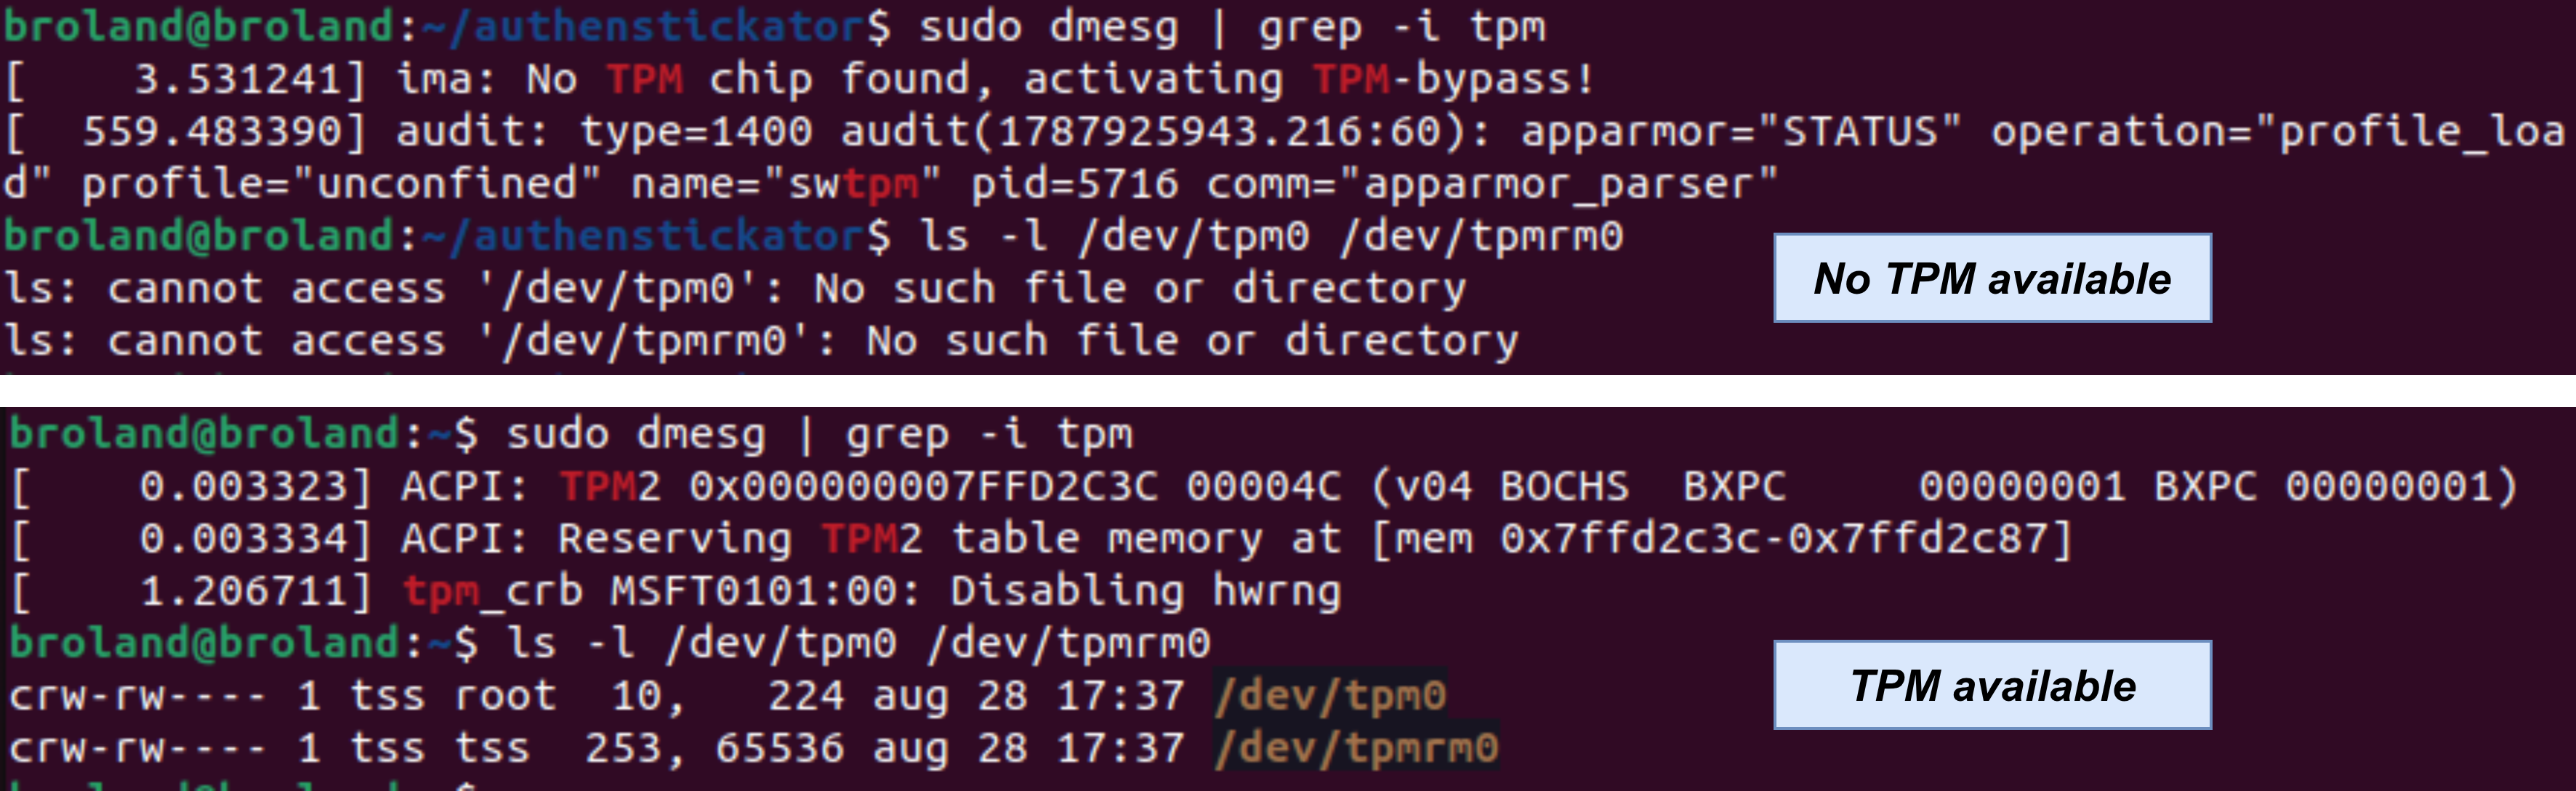
\includegraphics[width=\textwidth]{img/tpm-check.png}
    \caption{Check if you have a TPM.}
    \label{fig:tpm-check}
\end{figure}

For provisioning, you will need to run the \t{tss2\_provision} command of package \t{tpm2-tools}.
You can try getting it through \t{apt}, but it did not work for me.
\begin{lstlisting}[language=bash]
sudo apt install -y tpm2-tools
sudo -u tss tss2_provision
\end{lstlisting}

If you get a command not found error, welcome to the club.
The alternative is to compile \t{tpm2-tools} from source.
This package requires the \t{tpm2-tss} package, which also needs to be compiled from source with a compatible version.
I generated a script with Gemini, found in the repo under \t{script/setup\_fapi.sh}.
It can be run as shown in Listing \ref{lst:setup-fapi}.
This script:
\begin{enumerate}
  \item Installs dependencies for \t{tpm2-tss} and \t{tpm2-tools}.
  \item Adds your user to the \t{tss} group. You will run \app{} as your user, and interacting with TPM requires membership of this group.
  \item Compiles \t{tpm2-tss v4.1.3}.
  \item Compiles \t{tpm2-tools v5.6}.
  \item Removes some FAPI profiles which were too modern for Ubuntu 22.04 and adds \t{ek\_cert\_less = "yes"} to the automatically generated \t{fapi-config.json}.
  \item Creates the directories necessary for provisioning, and provisions.
  \item Generates a random number to see if TPM responds (although this does not require provisioning).
\end{enumerate}

\begin{lstlisting}[language=bash, label={lst:setup-fapi}, caption={Running the FAPI setup script.}]
chmod +x ./script/setup_fapi.sh
sudo ./script/setup_fapi.sh
\end{lstlisting}

If you mess with the TPM too much, it will lock you out.
TPM is protecting itself against dictionary attacks (DA), by disallowing further commands for a period of time.
This time period can be pretty long (don't ask me why I have this knowledge).
One possible solution to get out of the lockout is a command I found in a thread from Ubuntu\footnote{\url{https://documentation.ubuntu.com/core/how-to-guides/manage-ubuntu-core/troubleshooting/}}, shown in Listing \ref{lst:tpm-lockout}.
The file it modifies contained the value 0 when I was locked out, so it is probably a reversed violation counter.
Without a system reboot, the change has no effect.

\begin{lstlisting}[language=bash, label={lst:tpm-lockout}, caption={Getting out of TPM's Lockout Mode.}]
echo 5 | sudo tee /sys/class/tpm/tpm0/ppi/request
reboot
\end{lstlisting}

Also, if you get provisioning errors saying that TPM was already set up, you might want to try deleting previous keystores (see: Listing \ref{lst:wiping-keystores}).
These affect only FAPI, not the whole TPM (I have disk encryption which uses TPM, but this command did not break it).
If other software on your PC uses FAPI, you might want to look for a more graceful solution.

\begin{lstlisting}[language=bash, label={lst:wiping-keystores}, caption={Wiping previous keystores.}]
sudo rm -r /var/lib/tpm2-tss/system/keystore/
rm -r ~/.local/share/tpm2-tss/user/keystore/
\end{lstlisting}

The default \t{fapi\_config} is generated while compiling tpm2-tss and tpm2-tools.
It can be found at the path \t{/etc/tpm2-tss/fapi-config.json}.
After the script's modifications, it might look like on Listing \ref{lst:default-fapi-config}.
\begin{lstlisting}[language=json, label={lst:default-fapi-config}, caption={The default \t{fapi-config.json}, after the script's modifications.}]
{
  "profile_name": "P_ECCP256SHA256",
  "profile_dir": "/etc/tpm2-tss/fapi-profiles/",
  "user_dir": "~/.local/share/tpm2-tss/user/keystore",
  "system_dir": "/var/lib/tpm2-tss/system/keystore",
  "tcti": "",
  "system_pcrs": [],
  "log_dir": "/var/run/tpm2-tss/eventlog/",
  "firmware_log_file": "/sys/kernel/security/tpm0/binary_bios_measurements",
  "ima_log_file": "/sys/kernel/security/ima/binary_runtime_measurements",
  "ek_cert_less": "yes"
}
\end{lstlisting}

\subsubsection{Virtual TPM}

To run with a virtual TPM, change the configs to enable it (see: Section \ref{lab:ch4-config}).
It should work out of the box.
But if you have to troubleshoot, you can check manually if \t{swtpm} is running using \t{netcat} (see: Listing \ref{lst:check-swtpm}).
While \app{} runs, the command should output something like ``Connection to localhost (127.0.0.1) 2322 port [tcp/*] succeeded!''.
Run it multiple times, the first one might fail.
Make sure the ports match the ones in configs.
\begin{lstlisting}[language=bash, label={lst:check-swtpm}, caption={Checking if the virtual TPM is running.}]
nc -zv localhost 2322
\end{lstlisting}

If \t{swtpm} locks you out and/or you want to start fresh, you can kill its process and delete its folder.
\begin{lstlisting}[language=bash]
pkill swtpm | rm -r /tmp/vtpm
\end{lstlisting}

Then, you can re-launch the app, or run the commands from \t{linux\_tpm.py} manually.



\subsection{Packing on Linux}

To pack \app{}, after a successful setup (see: Section \ref{lab:ch4-setup-on-linux}), run the Linux packing script, as in Listing \ref{lst:packing-linux}.
If you ran it previously, it will prompt you if you want to overwrite existing data, and you need to press Y.
The flags specified in \t{pack-linux.sh} add a name to the packed executable, add non-Python files which \t{pyinstaller} would not include by default, ensure paths start from root, and specify the output directory.
Builds are generated in the temporary folder, so they will be wiped at reboot; you can change this if you wish.

\begin{lstlisting}[language=bash, label={lst:packing-linux}, caption={Running the packing script for Linux.}]
source venv/bin/activate
pip install pyinstaller
./script/pack-linux.sh
\end{lstlisting}

If you want to create a release/archive, navigate to the previous command's output (by default \t{/tmp/authenstickator/dist}) and pack it using \t{tar}.
See Listing \ref{lst:archive-linux} for an example of packing for an Ubuntu release, and later extracting.
If you did this on a VM and want to get the archive to your host machine, on the VM, you can get your IP (\t{YOUR-VM-IP}) using \t{ip a}, then start a local HTTP server with Python using \t{python3 -m http.server 8000}.
After that, you can connect through your host's browser through \url{http://YOUR-VM-IP:8000/}.

\begin{lstlisting}[label={lst:archive-linux}, caption={Create archive and extract on Linux.}]
tar -czvf Authenstickator-v1.0.0-Ubuntu-22.04.5-LTS.tar.gz Authenstickator/
tar -xzvf Authenstickator-v1.0.0-Ubuntu-22.04.5-LTS.tar.gz
\end{lstlisting}



\subsection{Setup on Windows} \label{lab:ch4-setup-on-windows}

The following setup was tested on Microsoft Windows Version 10.0.19045.6466.
It might work on other Windows systems as well, but there is no guarantee.

Although development was done with Python 3.10.12, for Windows, this version does not have a binary release.
Instead, you can get 3.10.11 from \url{https://www.python.org/downloads/release/python-31011/}.
When running the installer, tick the option to add to path and to disable path length limit.
You will also need Git, you can get it from \url{https://git-scm.com/install/windows}.
After having Python and Git, run the commands from Listing \ref{lst:windows-setup}.
Command \t{where python} shall output as first entry \t{$\backslash$venv$\backslash$Scripts$\backslash$python.exe}; if not, try activating again/ in a new terminal (it happened to me).

\begin{lstlisting}[language=bash, label={lst:windows-setup}, caption={Setup commands for Windows.}]
git clone https://github.com/broland29/authenstickator.git
cd authenstickator
python -m venv venv
venv\Scripts\activate.bat
where python
pip install -r requirements.txt
\end{lstlisting}

If you get ``ImportError: DLL load failed while importing zxingcpp: The specified module could not be found.'', get \t{vc\_redist.x64.exe} from \url{https://aka.ms/vs/17/release/vc_redist.x64.exe}.

Once the scripts from \ref{lst:windows-setup} all finished, you can start the app.
Always activate the virtual environment before running.
\begin{lstlisting}[language=bash, label={lst:linux-run-app}, caption={Running the app on Linux.}]
python -m src.main
\end{lstlisting}

To ensure that the app is properly working, you can run the unit tests:
\begin{lstlisting}[language=bash, label={lst:linux-run-tests}, caption={Running the tests on Linux.}]
python -m pytest
\end{lstlisting}



\subsubsection{Packing on Windows}

To pack \app{}, after a successful setup (see: Section \ref{lab:ch4-setup-on-windows}), run the Windows packing script, as in Listing \ref{lst:packing-windows}.
If you ran it previously, it will prompt you if you want to overwrite existing data, and you need to press Y.
The flags specified in \t{pack-windows.bat} add a name and icon to the packed executable, add non-Python files which \t{pyinstaller} would not include by default, ensure paths start from root, disable the scary black terminal, and specify the output directory.
Builds are generated in the temporary folder; you can change this if you wish.

\begin{lstlisting}[language=bash, label={lst:packing-windows}, caption={Running the packing script for Windows.}]
venv\Scripts\activate.bat
pip install pyinstaller
script\pack-windows.bat
\end{lstlisting}


If you want to create a release/archive, navigate to the previous command's output (by default \t{C:$\backslash$Users$\backslash$YOUR-USERNAME$\backslash$AppData$\backslash$Local$\backslash$Temp$\backslash$authenstickator$\backslash$dist}) and pack it using \t{tar}.
See Listing \ref{lst:archive-linux} for an example of packing for an Ubuntu release, and later extracting.
If you did this on a VM and want to get the archive to your host machine, on the VM, you can get your IP (\t{YOUR-VM-IP}) using \t{ipconfig}, then start a local HTTP server with Python using \t{python -m http.server 8000
}.
After that, you can connect through your host's browser through \url{http://YOUR-VM-IP:8000/}.

\begin{lstlisting}[label={lst:archive-windows}, caption={Create archive and extract on Windows.}]
tar -a -c -f Authenstickator-v1.0.0-Windows-10.zip Authenstickator
tar -x -f Authenstickator-v1.0.0-Windows-10.zip
\end{lstlisting}

As the output says, the result is in your temporary folder, by default \t{C:\\Users\\YOURUSERNAME\\AppData\\Local\\Temp\\authenstickator\\dist}.




\section{User Manual}

\subsection{USB Setup on Linux}

\subsection{USB Setup on Windows}






\subsection{App functionalities}
